\scanpage{20}
Ainsi les classes de $\Pi_I^{\unsure{\circ|0}}$ sont les classes de $\Pi_J^\circ$ distinctes de $\deleted{\Pi}U_{J,i}$, et de plus les \unsure{clas.|deux.} parmi
\[
U_{J,i}\cap\Sigma_{\unsure{\deleted{J}i|j|i}}^+,\quad U_{J,i}\cap\Sigma_i^-
\]
qui sont non vides. Or les deux classes en question sont non vides, car
% B_G01: cancelled Sigma and its two visible crossing runs. Observed locus (320,810,403,900).
% Source origin (315,803); x right, y down; 0.25 pt per source pixel. Baseline y=76.
% The visible node occurs once; its phantom carries the deletion state without a generic extra rule.
\begin{tikzpicture}[x=0.25pt,y=-0.25pt,baseline={(0,76)}]
\path[use as bounding box] (0,0) rectangle (95,100);
\node[anchor=base west,inner sep=0pt,outer sep=0pt] at (4,76) {\rlap{$\unsure{\Sigma_j|\Sigma_i}$}\phantom{\deleted{$\unsure{\Sigma_j|\Sigma_i}$}}};
\draw[line width=0.45pt,line cap=round] (10,73) .. controls (20,54) and (30,31) .. (40,12);
\draw[line width=0.45pt,line cap=round] (45,73) .. controls (43,80) and (49,82) .. (54,76) -- (69,35);
\end{tikzpicture}
$U_{J,i}$ est un voisinage de $\deleted{\Sigma}E_{\unsure{i|j}}$, et
\[
\overline{\Sigma_i^+}\cap\deleted{\Sigma}E_i\ne\varnothing,\quad
\overline{\deleted{E}\Sigma_i^-}\cap\deleted{\Sigma}E_i\ne\varnothing.
\]
On sait donc que le nb des classes est en \deleted{\unsure{tout|est}} $(n-1)+2=n+1=\operatorname{card} I+1$ (ce qui achève \unsure{aussi|ainsi}
% B_G02: complete word-bearing group la and one qualified detached point above/right.
% Origin (500,1347), 0.25 pt per source pixel, baseline y=49. Observed point locus (566,1363,575,1373).
% Inner graphic origin is explicitly translated by (66,18); base-west anchor and baseline (0,0) fix its placement.
\begin{tikzpicture}[x=0.25pt,y=-0.25pt,baseline=(Bla.base)]
\path[use as bounding box] (0,0) rectangle (88,62);
\node[anchor=base west,inner sep=0pt,outer sep=0pt] (Bla) at (0,49) {la};
\node[anchor=base west,inner sep=0pt,outer sep=0pt] at (66,18) {\unsure{\begin{tikzpicture}[x=0.25pt,y=-0.25pt,baseline={(0,0)}]
\path[use as bounding box] (0,0) rectangle (7,8);
\fill (2,0) -- (5,4) -- (4,7) -- (1,6) -- cycle;
\end{tikzpicture}}};
\end{tikzpicture}
\unsure{dèm.|dém.|dem.} par récurrence sur le nb des classes).

\uline{Lemme} Toute classe de $\Pi_I^\circ$ est de la forme
% B_G03: union, complete parenthesized expression, overwritten limit, raised hatted Sigma, and literal brace.
% Origin (1010,1600), 0.25 pt per source pixel, baseline y=140; fixed drawing rectangle (0,15)-(390,200).
% Pi above and X setminus to the left are outside this group. No generic bigcup or overbrace is also drawn.
$X\setminus\text{\begin{tikzpicture}[x=0.25pt,y=-0.25pt,baseline={(0,140)}]
\path[use as bounding box] (0,15) rectangle (390,200);
% U01 body; U02 upper-right loop; U03 pale lower retrace.
\draw[line width=0.95pt,line cap=round] (17,90) .. controls (17,122) and (24,140) .. (45,142) .. controls (63,142) and (72,133) .. (71,115) -- (68,87);
\draw[line width=0.55pt,line cap=round] (68,87) .. controls (66,77) and (63,81) .. (64,89) .. controls (65,96) and (68,99) .. (68,104);
\draw[black!55,line width=0.45pt,line cap=round] (19,114) .. controls (23,140) and (51,150) .. (65,133);
\node[anchor=base west,inner sep=0pt,outer sep=0pt,font=\small] at (0,190) {$\alpha\in\unsure{\deleted{I}K|K}$};
\node[anchor=base west,inner sep=0pt,outer sep=0pt,font=\small] at (91,140) {$(\Sigma_\alpha^+\cup E_\alpha)$};
\node[anchor=base west,inner sep=0pt,outer sep=0pt,font=\scriptsize] at (184,58) {$\inserted{\widehat{\Sigma}_\alpha^+}$};
% BR01 main run and central turn; BR02 closed left loop; BR03 left retrace.
\draw[line width=0.65pt,line cap=round] (108,79) .. controls (132,75) and (151,71) .. (180,74) .. controls (193,75) and (204,70) .. (217,72) -- (220,62) .. controls (234,70) and (256,68) .. (287,64) .. controls (307,60) and (326,59) .. (339,62) .. controls (344,63) and (345,66) .. (345,69);
\draw[line width=0.55pt,line cap=round] (132,76) .. controls (141,68) and (160,69) .. (164,74) .. controls (153,81) and (142,82) .. (132,76);
\draw[line width=0.85pt,line cap=round] (120,80) .. controls (145,74) and (178,73) .. (210,74);
\end{tikzpicture}}$
où $K$ est une
% B_G04 contains exactly partie, the inserted/deleted non vide, and de I, et.
% Source origin (997,1750), 0.25 pt per source pixel, baseline y=110. Fixed rectangle (0,0)-(530,160).
% NV01 is the rising cancellation run with its right return. NV02 is the separate curved insertion guide.
\begin{tikzpicture}[x=0.25pt,y=-0.25pt,baseline={(0,110)}]
\path[use as bounding box] (0,0) rectangle (530,160);
\node[anchor=base west,inner sep=0pt,outer sep=0pt] at (0,115) {partie};
\node[anchor=base west,inner sep=0pt,outer sep=0pt,font=\small,rotate=8] at (157,45) {\inserted{\rlap{non vide}\phantom{\deleted{non vide}}}};
\node[anchor=base west,inner sep=0pt,outer sep=0pt] at (200,89) {de $I$, et};
\draw[line width=0.55pt,line cap=round] (154,53) .. controls (203,44) and (282,30) .. (331,24) .. controls (331,31) and (325,37) .. (315,43);
\draw[line width=0.45pt,line cap=round] (182,94) .. controls (172,61) and (272,47) .. (339,40) .. controls (346,39) and (351,39) .. (355,43);
\end{tikzpicture}
% slanted; the two written conditions have no punctuation between them.
\reversemarginpar\margin{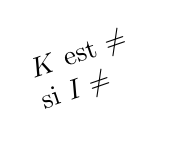
\begin{tikzpicture}\node[rotate=19,anchor=base west,inner sep=0pt,outer sep=0pt] {\shortstack[l]{$K$ est $\ne\varnothing$\\si $I\ne\varnothing$}};\end{tikzpicture}}\normalmarginpar
$\forall\alpha\in K$, \deleted{on a} $\Sigma_\alpha^+
% B_G05 literal reworked relation, followed inside the qualifier by its supported complete-state interpretations.
% Origin (943,1947), 0.25 pt per source pixel, baseline y=43; observed locus (944,1949,999,2004).
% M01 curved body, M02 middle shaft, M03 thin right head. No additional unqualified membership or arrow is drawn.
\mathrel{\unsure{\text{\begin{tikzpicture}[x=0.25pt,y=-0.25pt,baseline={(0,43)}]
\path[use as bounding box] (0,0) rectangle (62,66);
\draw[line width=0.70pt,line cap=round] (45,11) .. controls (35,-1) and (16,17) .. (7,32) .. controls (1,43) and (5,51) .. (15,55) .. controls (23,58) and (32,56) .. (39,51);
\draw[line width=0.75pt,line cap=round] (4,40) -- (43,32);
\draw[line width=0.40pt,line cap=round] (35,24) .. controls (38,16) and (51,29) .. (54,36) .. controls (56,34) and (54,20) .. (48,19);
\end{tikzpicture}}|\deleted{\Rightarrow}\in|\deleted{\to}\in|\in}}
\pi_0(X\setminus E_\alpha)$, tels que $\forall\alpha,\beta\in K$, $\alpha\ne\beta$, on ait $\widehat{\Sigma}_\alpha^+\cap\widehat{\Sigma}_\beta^+=\varnothing$ $(\Longleftrightarrow\Sigma_\alpha^+\cap\Sigma_\beta^+=\varnothing)$.
% archive sheet number: 19
